
\documentclass[12pt]{scrreprt}
\usepackage{arbeitsblatt}
\usepackage{pifont}
\usepackage[left=1cm, right=2cm, bottom=2cm, top=2cm]{geometry}
\title{Installation von Git}
\ihead{Gitkurs}
\ohead{}
\setlength{\abovecaptionskip}{-15pt} 
\setlength{\belowcaptionskip}{10pt} 
\setlength{\parskip}{10pt} 
 
\begin{document} 
\section*{Bilderstrecke Git-Installation} 

\begin{miniseite}{7cm}
\begin{figure}[H]
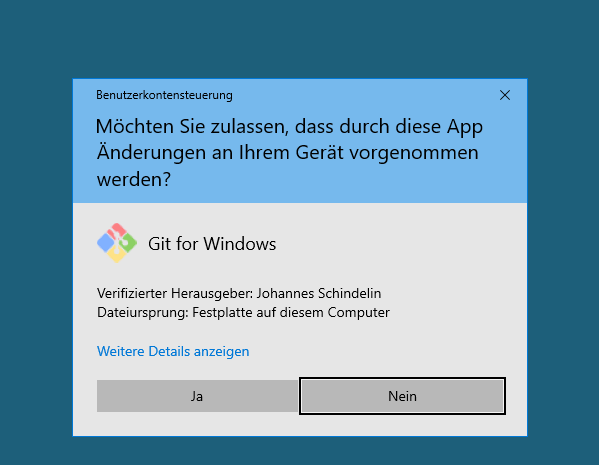
\includegraphics[width=8cm]{git_install_001.png}
\caption{Ja wählen}
\end{figure}
\end{miniseite}\hfill
\begin{miniseite}{7cm}
\begin{figure}[H]
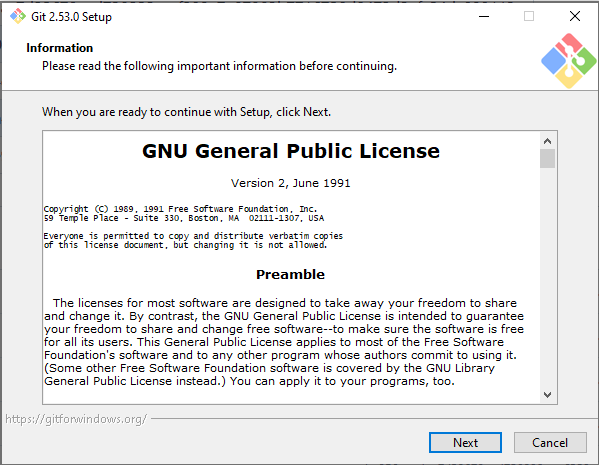
\includegraphics[width=8cm]{git_install_002.png}
\caption{Next wählen}
\end{figure}
\end{miniseite}


\begin{miniseite}{7cm}
\begin{figure}[H]
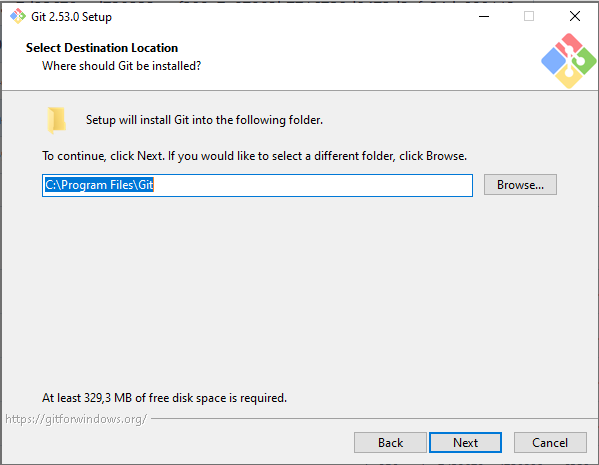
\includegraphics[width=8cm]{git_install_003.png}
\caption{Next wählen}
\end{figure}
\end{miniseite}\hfill
\begin{miniseite}{7cm}
\begin{figure}[H]
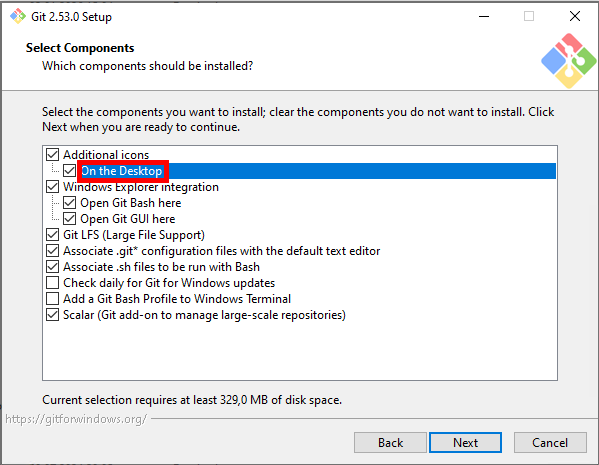
\includegraphics[width=8cm]{git_install_004.png}
\caption{Next wählen}
\end{figure}
\end{miniseite}


\begin{miniseite}{7cm}
\begin{figure}[H]
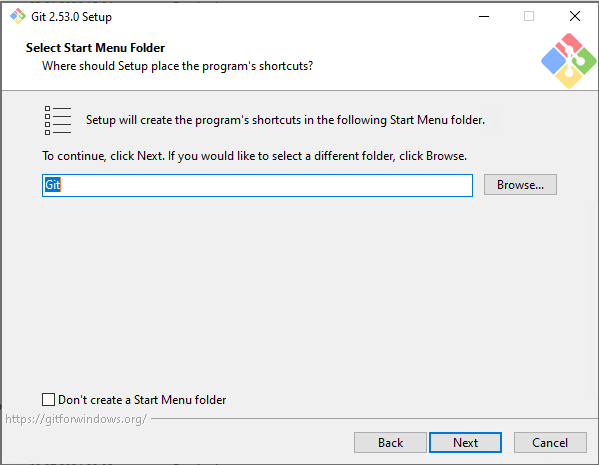
\includegraphics[width=8cm]{git_install_005.png}
\caption{Next wählen}
\end{figure}
\end{miniseite}\hfill
\begin{miniseite}{7cm}
\begin{figure}[H]
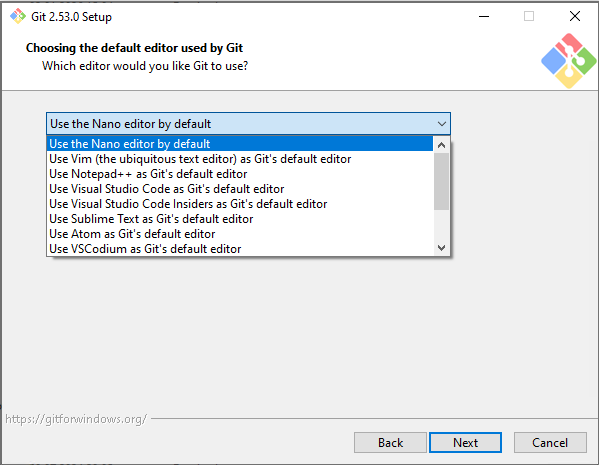
\includegraphics[width=8cm]{git_install_007.png}
\caption{Next wählen}
\end{figure}
\end{miniseite}

 
\begin{miniseite}{7cm}
\begin{figure}[H]
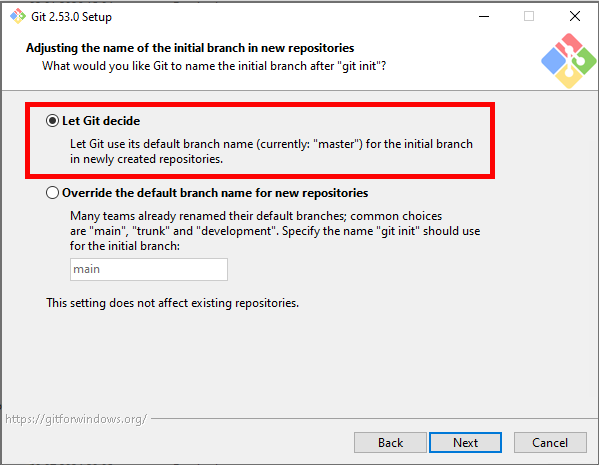
\includegraphics[width=8cm]{git_install_008.png}
\caption{Next wählen}
\end{figure}
\end{miniseite}\hfill
\begin{miniseite}{7cm}
\begin{figure}[H]
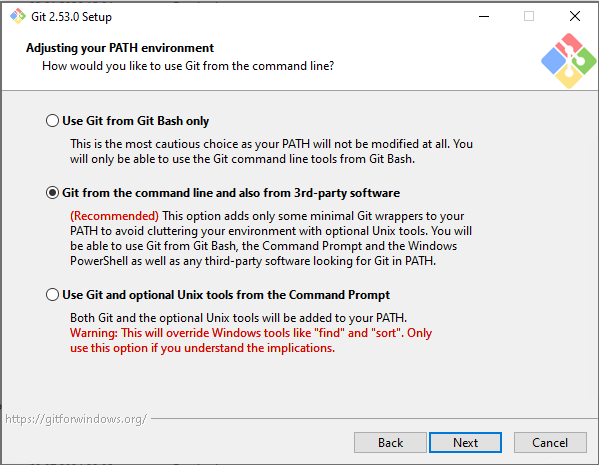
\includegraphics[width=8cm]{git_install_009.png}
\caption{Next wählen}
\end{figure}
\end{miniseite}


\begin{miniseite}{7cm}
\begin{figure}[H]
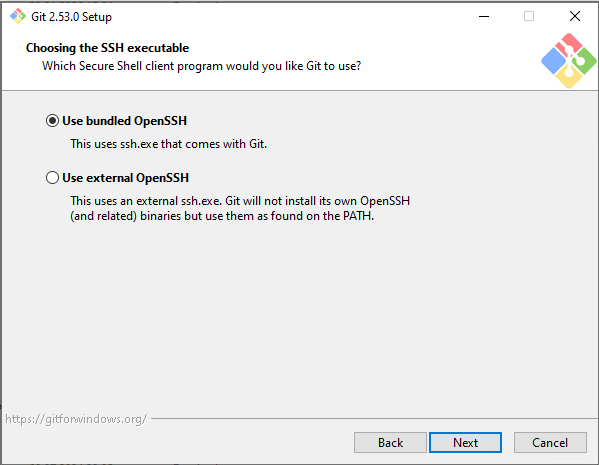
\includegraphics[width=8cm]{git_install_010.png}
\caption{Next wählen}
\end{figure}
\end{miniseite}\hfill
\begin{miniseite}{7cm}
\begin{figure}[H]
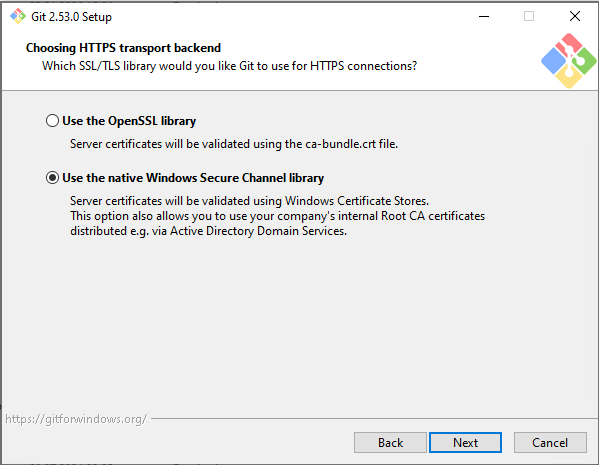
\includegraphics[width=8cm]{git_install_011.png}
\caption{Next wählen}
\end{figure}
\end{miniseite}


\begin{miniseite}{7cm}
\begin{figure}[H]
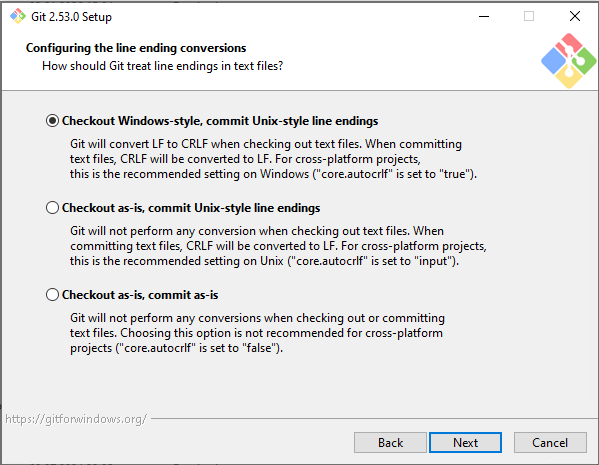
\includegraphics[width=8cm]{git_install_012.png}
\caption{Next wählen}
\end{figure}
\end{miniseite}\hfill
\begin{miniseite}{7cm}
\begin{figure}[H]
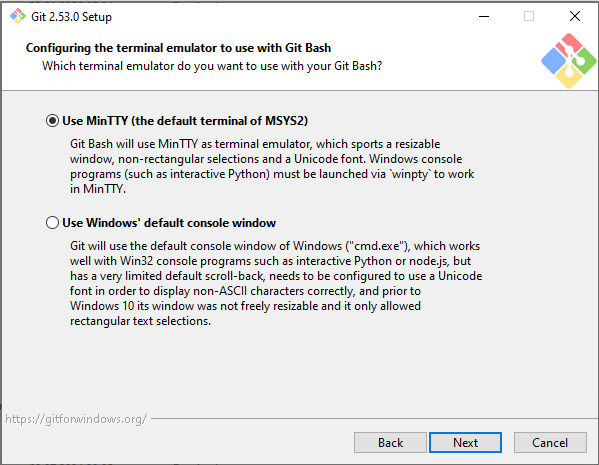
\includegraphics[width=8cm]{git_install_013.png}
\caption{Next wählen}
\end{figure}
\end{miniseite}



\begin{miniseite}{7cm}
\begin{figure}[H]
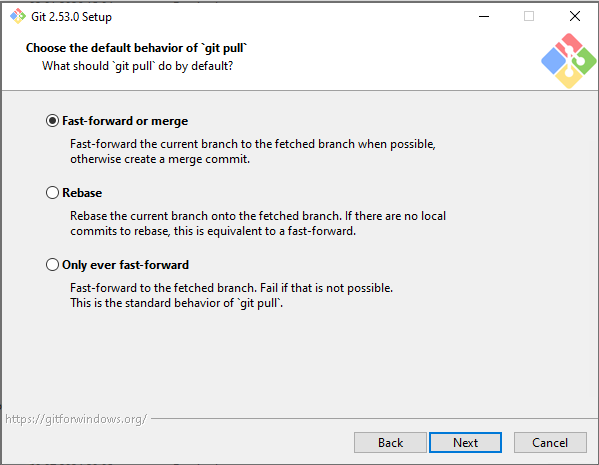
\includegraphics[width=8cm]{git_install_014.png}
\caption{Ja wählen}
\end{figure}
\end{miniseite}\hfill
\begin{miniseite}{7cm}
\begin{figure}[H]
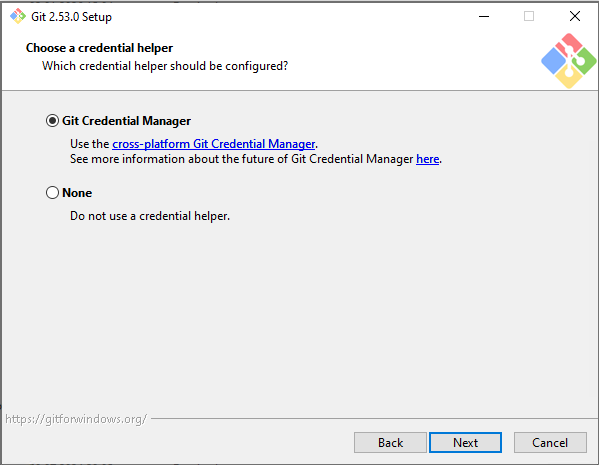
\includegraphics[width=8cm]{git_install_015.png}
\caption{Next wählen}
\end{figure}
\end{miniseite}

\begin{miniseite}{7cm}
\begin{figure}[H]
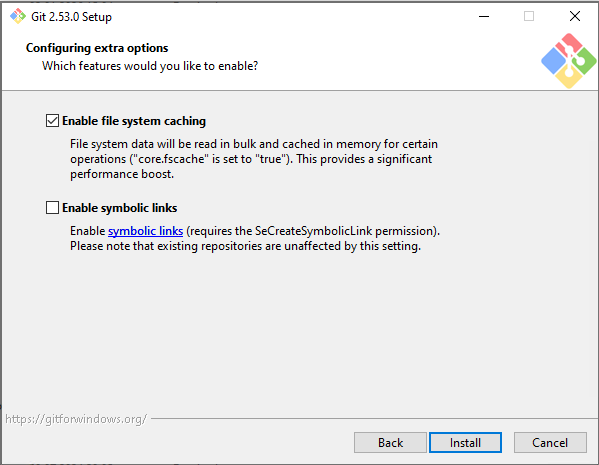
\includegraphics[width=8cm]{git_install_016.png}
\caption{Ja wählen}
\end{figure}
\end{miniseite}\hfill
\begin{miniseite}{7cm}
\begin{figure}[H]
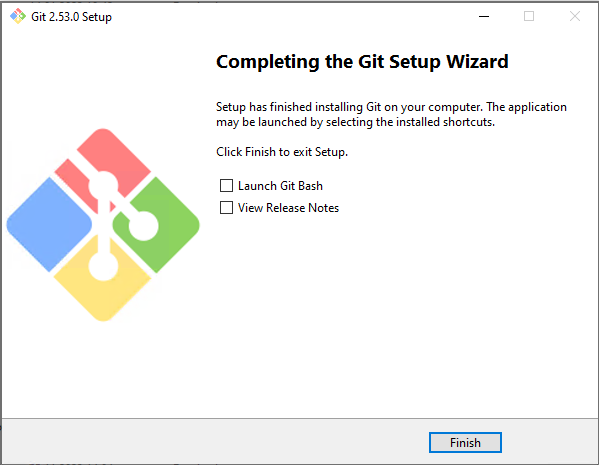
\includegraphics[width=8cm]{git_install_017.png}
\caption{Next wählen}
\end{figure}
\end{miniseite}

\end{document}
